%----------------------------------------------------------------------------------------
%	PACKAGES AND OTHER DOCUMENT CONFIGURATIONS
%----------------------------------------------------------------------------------------

\documentclass[a4paper,10pt,twoside]{article}
\usepackage[english]{babel}
\usepackage[utf8x]{inputenc}
\usepackage{amsmath}
\usepackage{graphicx}
\usepackage[colorinlistoftodos]{todonotes}
\usepackage{fancyhdr}
\usepackage[margin=0.97in]{geometry}

\setlength\paperheight{297mm}
\setlength\paperwidth{210mm}

\usepackage{avant}
\renewcommand{\familydefault}{\sfdefault}
\frenchspacing
 
\pagestyle{fancy}
\fancyhf{}
\fancyhead[LE,RO]{Project B Report}
\fancyhead[RE,LO]{Sakayan \textsc{Sitsabesan}}
\fancyfoot[RE,LO]{\today}
\fancyfoot[LE,RO]{\thepage}
 
\renewcommand{\headrulewidth}{2pt}
\renewcommand{\footrulewidth}{1pt}

\begin{document}

\begin{titlepage}

\newcommand{\HRule}{\rule{\linewidth}{0.5mm}} % Defines a new command for the horizontal lines, change thickness here

\center % Center everything on the page
 
%----------------------------------------------------------------------------------------
%	HEADING SECTIONS
%----------------------------------------------------------------------------------------

\textsc{\LARGE University of Auckland}\\[1.5cm] % Name of your university/college
\textsc{\Large COMPSYS 302: Design: Software Practice}\\[0.5cm] % Major heading such as course name
\textsc{\large Project B }\\[0.5cm] % Minor heading such as course title

%----------------------------------------------------------------------------------------
%	TITLE SECTION
%----------------------------------------------------------------------------------------

\HRule \\[0.4cm]
{ \huge \bfseries Final Report}\\[0.4cm] % Title of your document
\HRule \\[1.5cm]
 
%----------------------------------------------------------------------------------------
%	AUTHOR SECTION
%----------------------------------------------------------------------------------------

\begin{minipage}{0.4\textwidth}
\begin{flushleft} \large
\emph{Author:}\\
Sakayan \textsc{Sitsabesan}
\end{flushleft}
\end{minipage}
~
\begin{minipage}{0.4\textwidth}
\begin{flushright} \large
\emph{Supervisor:} \\
Mr. Andrew \textsc{Chen} % Supervisor's Name
\end{flushright}
\end{minipage}\\[1cm]


%----------------------------------------------------------------------------------------
%	DATE SECTION
%----------------------------------------------------------------------------------------

{\large \today}\\[2cm] % Date, change the \today to a set date if you want to be precise

%----------------------------------------------------------------------------------------
%	LOGO SECTION
%----------------------------------------------------------------------------------------


\includegraphics{uoa.png}\\[1cm] % Include a department/university logo - this will require the graphicx package
 
%----------------------------------------------------------------------------------------

\vfill % Fill the rest of the page with whitespace

\vspace*{25em}

{\Large Declaration of Originality}

\hspace{5em}

This report is my own unaided work and was not copied from 
nor written in collaboration with any other person.

Name: Sakayan \textsc{Sitsabesan}

\end{titlepage}

\section*{Acknowledgements}

I would like to thank our mentor, Andrew Chen, for guiding us throughout the semester with his constant help, supervision and suggestions. I would also like to thank him for his patience dealing with our numerous protocol issues and changes. Special mentions need to be made to Hammond Pearce and Micheal Orr for their ideas and assistance.

\newpage

\section{Developed System}

The second project for COMPSYS 302: Design: Software Practice involved making a peer-to-peer chat application. The client in this project is the CEO of a company who wishes for a program that enables secure encrypted chatting between the company's executive team. The main aim of this project was to create a reliable back end prototype system to meet these needs. The user interface was not a top priority but a significant amount of effort was put into make it as user friendly as possible. The system has been implemented in Python 2.7 using the CherryPy framework for creating the web interface of the application simpler.  The overall goals of the project were to:

\begin{itemize}
\item Allowing a user to log into the system
\item The system can automatically find other users on other computers
\item User can create and maintain a simple profile page
\item Users can send messages, images, audio, and PDF files to each other
\end{itemize}

In my implementation I have met all of these minimum requirements as well as going on to add special features such as Multiuser, Events co-ordination system, fallback p2p networking, offline messaging, markdown support, etc.

\section{Technology Stack}

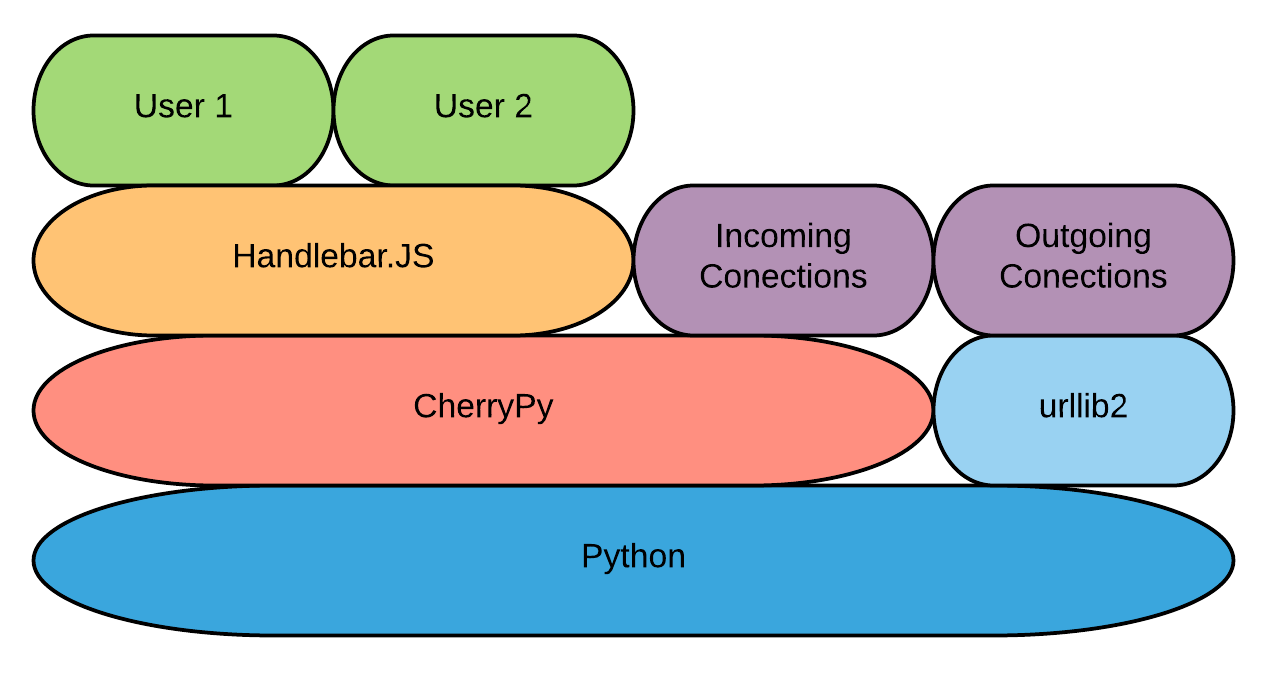
\includegraphics[width=1\textwidth]{tech_stack.png}

The main framework used in this project is CherryPy. This provides a web server and much of the tools needed to quickly implement a web app in Python. When the user open a web page on this server, CherryPy serves the template along with appropriate JS \& CSS files to the browser. On page load, AJAX calls are made back to the CherryPy server asking for the particular data to display on the screen at that moment. This data is returned as a list of dicts in JSON format. This is then rendered into place using the Handlebar.JS templating engine. Incoming connections to this node are handled directly by CherryPy whilst outgoing connections are initiated using urllib2.

\section{Issues faced during development}

A major issue faced during the development of the project was the difficulty in testing the components as they are developed. This is due to the very peer-to-peer nature of the project, where we are dependent on another peer being able to respond to our request correctly. This issue was much greater for me initially as I was one of the few that implemented most features first. For those that implemented them later, finding peers for testing was not as great of an issue. Multiple efforts were taken to counter this issue, one of these is working closely with other peers in the class to better align development and testing to make things easier. In addition debugging tools were used to go line-by-line through the Python code to better understand how the code was working. Fiddler, a HTTP debugging proxy, was also used to capture \& analyze the HTTP packets being sent \& received. HTTP packets could also be mocked from within this tool to emulate a real transaction when necessary. This issue was overcome through the use of these development tools and working more closely with other developers (classmates).

Another issue faced during development was the ambiguity of the protocol which was open to being interpreted differently by differing developers. This issue was resolved by working closely with the client to slowly agree on the exact details of the protocol and make it more clear. 

\section{Features}

\subsection{Multi user}

This node has been designed from the beginning to be a multi user node. This has been achieved with the help of CherryPy sessions. All userdata relevant to a user is stored in the CherryPy sessions data which is linked to a cookie on the users browser. This allows for multiple simultaneous sessions to operate on the same node.

\subsection{Two Factor Authentication}

Two factor authentication is enabled by default and can be turned off from the edit profile page. This works by generating a random 6 digit code and emailing it to the user, which has to be correctly entered into the system to complete the login process. This increases security and makes it harder for an infiltrator to login to the system.

\subsection{Events Coordination System}

An events coordination system has been added to this server. It allows for a basic event invitation to be sent to users and these users can send a reply indicating to the host about their attendance at that event. This makes this a convenient place for meetings and other events to be coordinated among the executive team at the client company.

\subsection{Fallback peer-to-peer Networking}

In the case of login server outage, this node will continue to report directly to all online nodes and share peer lists with them. The last reported public key will be used to communicate with these peers. This allows for short periods of login server outage to not affect the operation of the network. New nodes which use the same public-private keys will be able to join while the login server is out as this node stores last used public keys in its databases. On the other hand, this node uses a new public-private key for every session for increased security. As a result this node will not be able to merge into a fallback peer-to-peer network without the assistance of the login server.

\subsection{Multi-threading}

Multiple threads are used to allow multiple tasks to be simultaneously executed. Separate threads are used to get the peer list, report to the server, get peer profiles, get peer status. On startup a new thread is allocated to call /retrieveMessages on all the online users, after which this thread will exit. Whenever a message, file or event is sent the data is passed on to another daemon thread which handles the request and the calling thread will promptly respond to the user. This means the user doesn't have to wait for hashing, encryption, transmitting, etc. and the user can instead go on to do other things while this happens in the background.

\subsection{Forwarding of offline messages}

Whenever a message is sent, the destination is checked to see of it is currently in the peer list that has been retrieved from the login server every 60 seconds. If it is not there, then a copy of that message is forwarded on to every currently online node in the hope that one of them will kindly forward it to the destination at a later point when it is online. This node accepts all messages that are sent to its /receiveFile \& /receiveMessage API endpoints. Whenever a user calls /retrieveMessage on this node, all messages that are destined for that user that have not already been sent to it will be forwarded to it. This allows this node to both be a relay and use other relay nodes to allow for offline messaging when a destination user if offline.

\subsection{Encryption \& Hashing}

As the protocol allowed for a large variation in hashing and encryption standards, in this project I aimed to support all of them. This was because I wanted for this node to be able to communicate with all the nodes developed in the class. To this end, all encryption and hashing standards have been implemented in this node. Hashing using bcrypt \& scrypt are much slower than the SHA256 or SHA512 especially with large attachments. This might be because the aim of bcrypt / scrypt is for password hashing and not exactly for general purpose integrity checking like its being used here. The limitations of block ciphers like RSA were also discovered when implementing this protocol. For example with RSA 1024, messages were limited to 1024bits or 128 characters of ASCII. This limitation was overcome by encrypting the key for a stream cipher using the block cipher and then encrypting the message using the stream cipher. This was how encryption level 4 of the protocol works, this is the preferred encryption standard in this project. When sending a message, the destinations listAPI is called and parsed to find out what hashing \& encryption standards are supported by the destination and these are used to send the message.

\subsection{Formatted messages}

All messages sent and received by this server are capable of transmitting markdown formatted text. This enables users to send things such as bold, italics, bullet points, etc. with their text. Markdown was used instead of HTML injection, as this could possibly open up security vulnerabilities in the system. Text messages received are passed through the Markdown 2.6 Python package which convert markdown syntax into HTML syntax. When messages are being sent, the SimpleMDE JS text editor that has been embedded can be used to edit and compose messages using Markdown syntax using a GUI. Alternatively users who are well versed in markdown can just start typing messages with markdown syntax, and it will be correctly rendered in the editor.

\section{Peer to Peer Methods}

In a central server model all the traffic goes through the central server, this allows for full storage of messages for offline users and easy monitoring of user permissions. This central server is also a huge vulnerability as a copy of all data is available on this server and if it is compromised all the data on it can be accessed by an attacker. This goes against the very needs of the client for this project.

On the other hand in a pure peer to peer model, all traffic goes from peer directly to the destination peer or through intermediate peers. In this system, intermediate peers should not be storing traffic that goes through them, and therefore only data relevant to a particular user will be stored on their computer. This means there is no central server that could easily be compromised to easily loose all the data. Instead an attacker must attack each and every peer to gain access to all the data that has been processed through this network. The only issue with this is the fact that finding the IP addresses of peers on start up is difficult and the difficulty in authenticating users into the network.

As both these models have their benefits and disadvantages, in our project we decided to make a hybrid of these two methods. This is where there is a central login server which authenticates the users and maintains a peer list of everyone's IP \& public keys. This means that communication data can remain peer to peer. This hybrid model takes the benefits from both models without many of the disadvantages. The only disadvantage that remains is that if the login server were to go down, the network will become unusable. This has been overcome in this project by having a fallback pure peer to peer network, where connections with the other peers are maintained when the login server goes down.

\section{Suitability of the Protocol}

The protocol that was used in the final project was very suitable for this project. All messages were JSON encoded to make parsing and processing the data more straightforward. The protocol was too flexible to allow for all the students in the class be able to work with it. Things like optional time stamps were initially an annoyance that was rectified in later iterations of the protocol. 

\section{Protocol Development Process}

The protocol development process was very much involved for all parties and was done in such a manner to cater to the needs of all the students in the class. Initially groups of three to ten students put together protocol proposals and submitted them to the client for review. These protocols were reviewed by the client and then a discussion among the developers took place. Following the discussion the decision to make a peer to peer protocol with a central login server was chosen. Afterwards a basic initial official protocol was released by the client. As we worked along and implemented sections of the code, any changes that were deemed necessary were incorporated into the protocol. Protocol for additional special features was also drafted, discussed and added to the official protocol with the support of developers.

\section{Suitability of Tools used}

The tools used in this project were very appropriate and suitable for this project. Python is a high level scripting language with much usage in the Linux and Academic communities. It has an extensive collection of in-built modules which can be imported to achieve almost anything. Python also support multiple programming paradigms including functional, procedural \& object-oriented. A mixture of these were used in this project to achieve the best result within the limited time frame for this project. The web framework used for this project is also quite suitable as it abstracts the web interfacing away from the developer without placing too many restrictions on the programmer's freedom. 

\section{Suggested Improvements}

Improvements for next time include Unit Testing, Automatic Refreshing, group conversations and searching features. Unit Testing is the software development process where the small units of the code are independently and individually tested for correct operation. As this is only a prototype and because of the short space of time over which this project was developed, this project doesn't use any unit tests. This could be fixed in the future with the addition of unit testing that covers a majority of the code base. 

Automatic refreshing of the pages as new messages come in was not implemented in this project. As the front end development was not of major concern to this project, it was also not implemented. Another related improvement is the addition of notifications so that the operator of the program is informed when new messages are received.

The addition of a group conversations feature will allow members of the executive team to take part in one group conversation online. Whether group conversations will be an appreciated feature at the client's company is unknown. A searching functionality can be also be added to the front end at a future point, this would reduce the endless scrolling a user might need to do to find some information they wanted to find.

\section*{Appendices}

\subsection*{Some screenshots of the Application}

\begin{center}

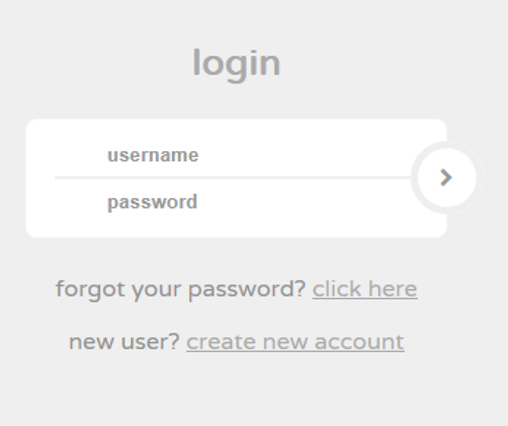
\includegraphics[width=0.5\textwidth]{appendix1.png}\\


\includegraphics[width=0.5\textwidth]{appendix2.png}\\

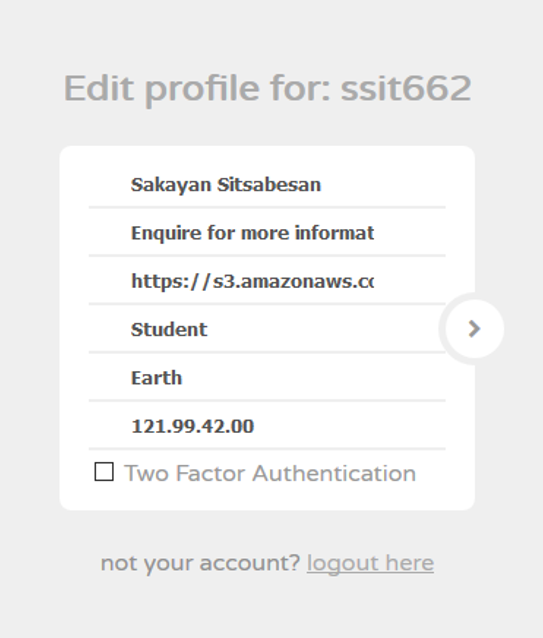
\includegraphics[width=0.5\textwidth]{appendix3.png}\\

\newpage

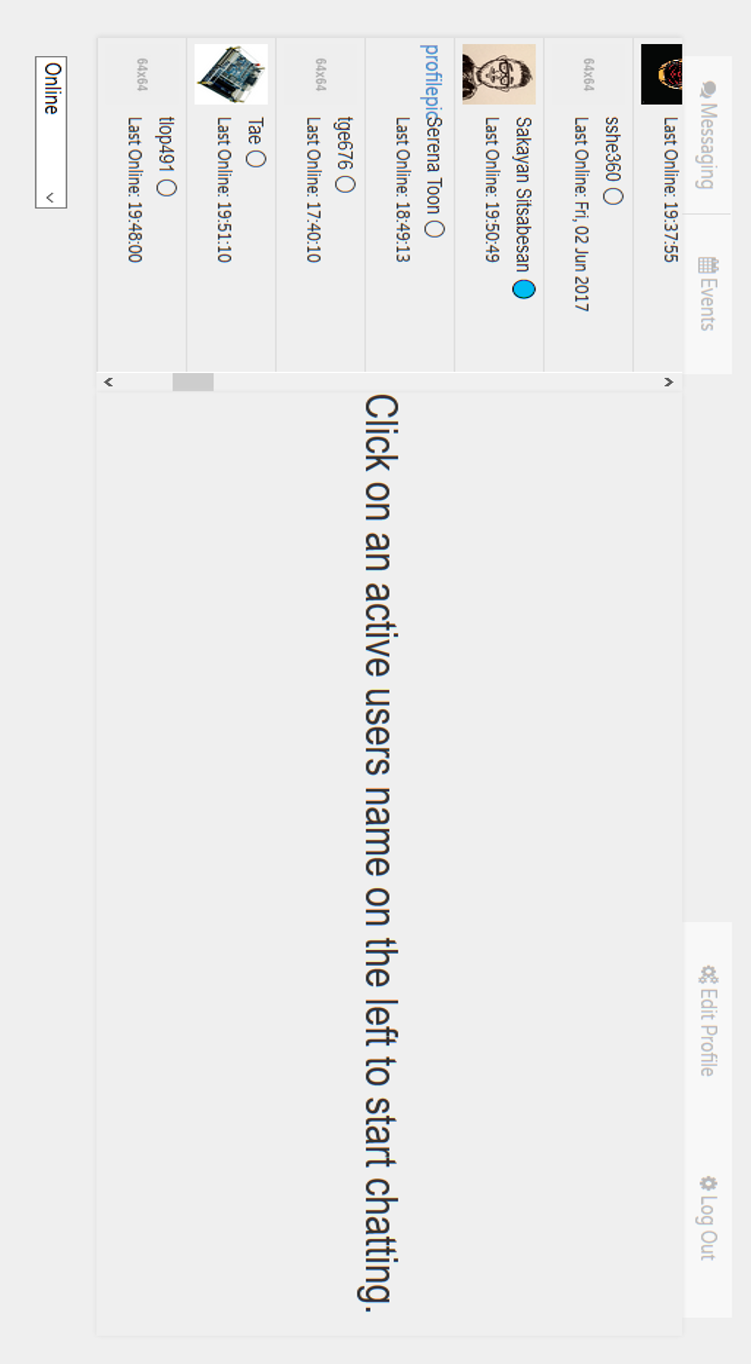
\includegraphics[width=0.75\textwidth]{appendix4.png}

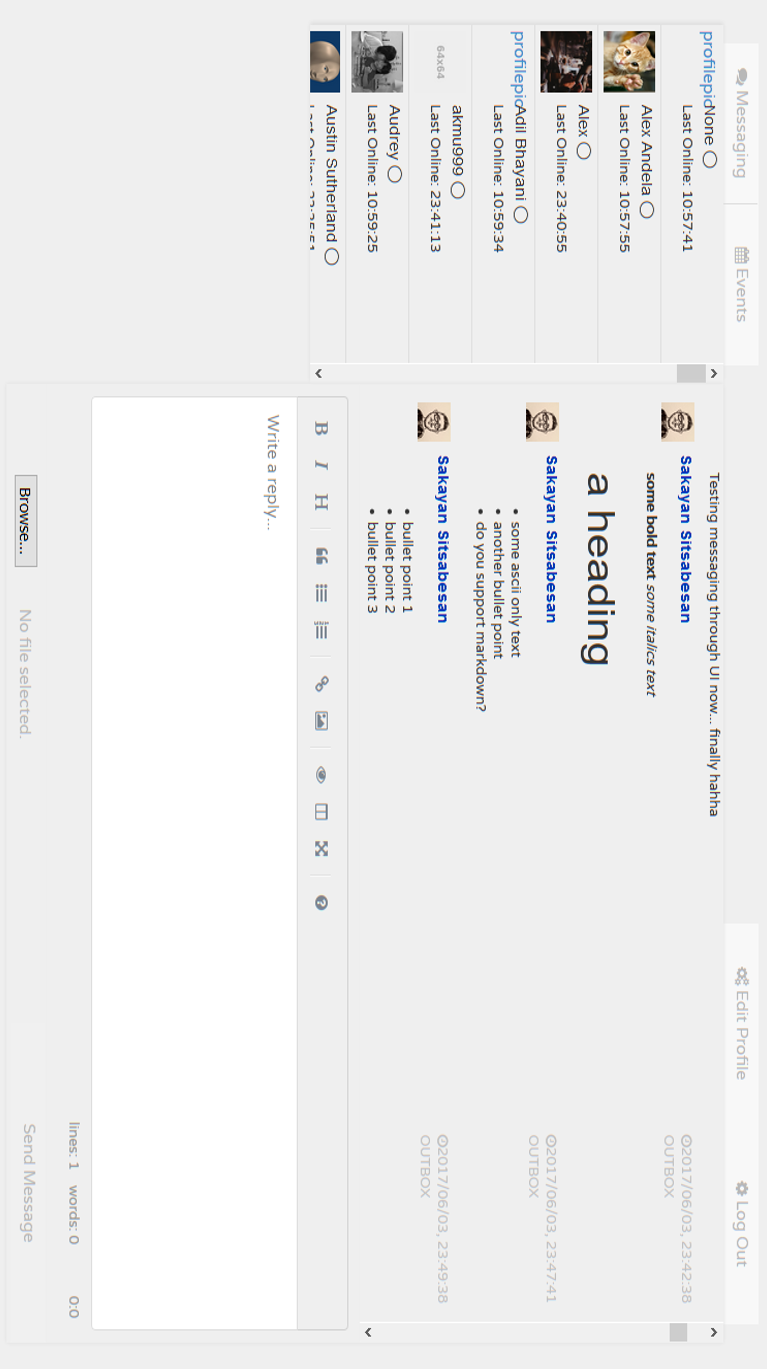
\includegraphics[width=0.75\textwidth]{appendix5.png}

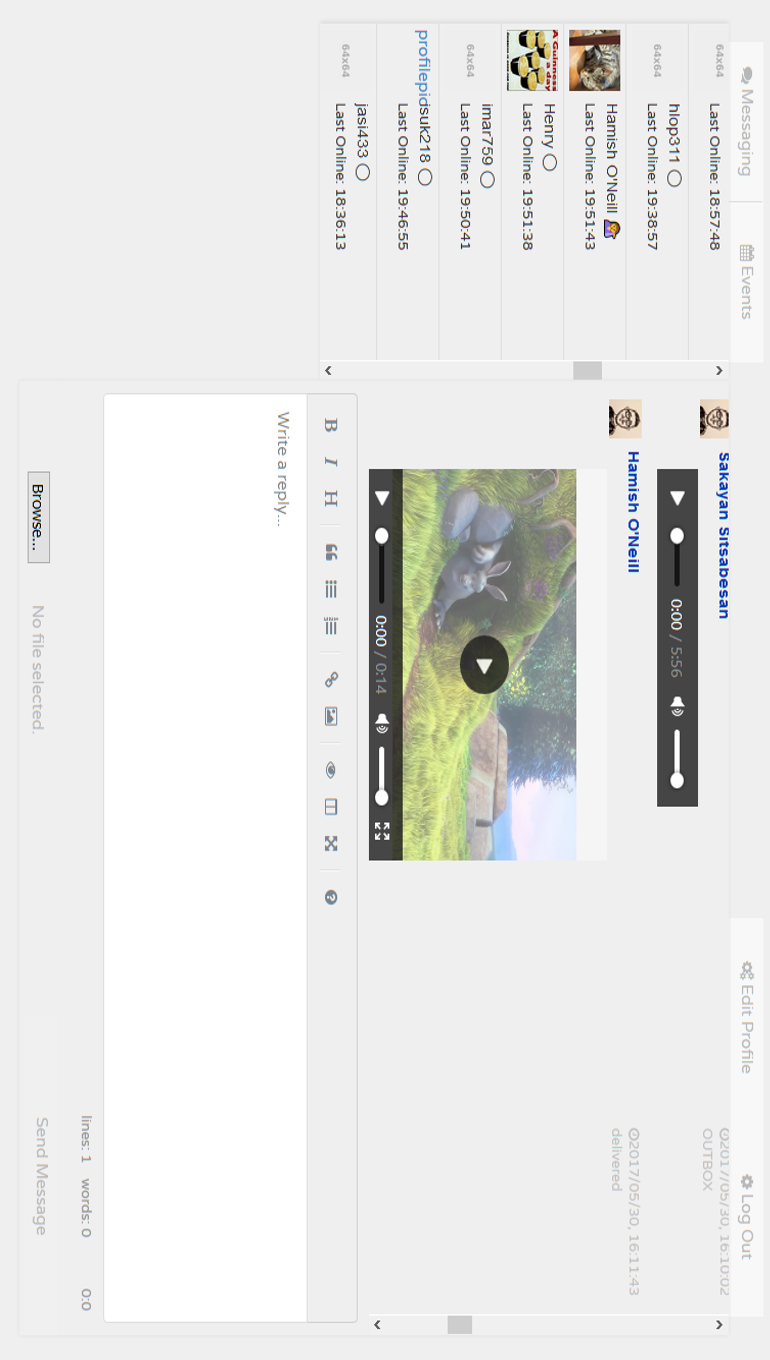
\includegraphics[width=0.75\textwidth]{appendix6.png}

\end{center}

\newpage
\mbox{}
\newpage

\end{document}